% Options for packages loaded elsewhere
\PassOptionsToPackage{unicode}{hyperref}
\PassOptionsToPackage{hyphens}{url}
\documentclass[
  ignorenonframetext,
]{beamer}
\newif\ifbibliography
\usepackage{pgfpages}
\setbeamertemplate{caption}[numbered]
\setbeamertemplate{caption label separator}{: }
\setbeamercolor{caption name}{fg=normal text.fg}
\beamertemplatenavigationsymbolsempty
% remove section numbering
\setbeamertemplate{part page}{
  \centering
  \begin{beamercolorbox}[sep=16pt,center]{part title}
    \usebeamerfont{part title}\insertpart\par
  \end{beamercolorbox}
}
\setbeamertemplate{section page}{
  \centering
  \begin{beamercolorbox}[sep=12pt,center]{section title}
    \usebeamerfont{section title}\insertsection\par
  \end{beamercolorbox}
}
\setbeamertemplate{subsection page}{
  \centering
  \begin{beamercolorbox}[sep=8pt,center]{subsection title}
    \usebeamerfont{subsection title}\insertsubsection\par
  \end{beamercolorbox}
}
% Prevent slide breaks in the middle of a paragraph
\widowpenalties 1 10000
\raggedbottom
\AtBeginPart{
  \frame{\partpage}
}
\AtBeginSection{
  \ifbibliography
  \else
    \frame{\sectionpage}
  \fi
}
\AtBeginSubsection{
  \frame{\subsectionpage}
}
\usepackage{iftex}
\ifPDFTeX
  \usepackage[T1]{fontenc}
  \usepackage[utf8]{inputenc}
  \usepackage{textcomp} % provide euro and other symbols
\else % if luatex or xetex
  \usepackage{unicode-math} % this also loads fontspec
  \defaultfontfeatures{Scale=MatchLowercase}
  \defaultfontfeatures[\rmfamily]{Ligatures=TeX,Scale=1}
\fi
\usepackage{lmodern}
\ifPDFTeX\else
  % xetex/luatex font selection
\fi
% Use upquote if available, for straight quotes in verbatim environments
\IfFileExists{upquote.sty}{\usepackage{upquote}}{}
\IfFileExists{microtype.sty}{% use microtype if available
  \usepackage[]{microtype}
  \UseMicrotypeSet[protrusion]{basicmath} % disable protrusion for tt fonts
}{}
\makeatletter
\@ifundefined{KOMAClassName}{% if non-KOMA class
  \IfFileExists{parskip.sty}{%
    \usepackage{parskip}
  }{% else
    \setlength{\parindent}{0pt}
    \setlength{\parskip}{6pt plus 2pt minus 1pt}}
}{% if KOMA class
  \KOMAoptions{parskip=half}}
\makeatother
\usepackage{longtable,booktabs,array}
\usepackage{caption}
\captionsetup[table]{skip=6pt}
\newcounter{none} % for unnumbered tables
\usepackage{calc} % for calculating minipage widths
\usepackage{caption}
% Make caption package work with longtable
\makeatletter
\def\fnum@table{\tablename~\thetable}
\makeatother
\usepackage{graphicx}
\makeatletter
\newsavebox\pandoc@box
\newcommand*\pandocbounded[1]{% scales image to fit in text height/width
  \sbox\pandoc@box{#1}%
  \Gscale@div\@tempa{\textheight}{\dimexpr\ht\pandoc@box+\dp\pandoc@box\relax}%
  \Gscale@div\@tempb{\linewidth}{\wd\pandoc@box}%
  \ifdim\@tempb\p@<\@tempa\p@\let\@tempa\@tempb\fi% select the smaller of both
  \ifdim\@tempa\p@<\p@\scalebox{\@tempa}{\usebox\pandoc@box}%
  \else\usebox{\pandoc@box}%
  \fi%
}
% Set default figure placement to htbp
\def\fps@figure{htbp}
\makeatother
\setlength{\emergencystretch}{3em} % prevent overfull lines
\providecommand{\tightlist}{%
  \setlength{\itemsep}{0pt}\setlength{\parskip}{0pt}}
% Manuscript macro/package fallbacks (newcommand -> providecommand).
\usepackage{amsmath}
\usepackage{amssymb}
\usepackage{booktabs}
% Contents listing: article.cls prefixes every \l@section entry with
% \addvspace{1.0em}, which across ten sections costs about ten lines and pushed
% the ~40-entry listing one line past page 2 — leaving a third sheet carrying a
% single "10 References" line. Tighten that inter-section gap for the duration
% of \tableofcontents only, inside a group, so body spacing is untouched and no
% entry is dropped (reducing \tocdepth would have hidden 29 real subsections).
  \providecommand{\addvspace}[1]{\vskip 2\p@}%
% Document metadata. config.yaml declares a subtitle and a keyword list, and
% the producer emits both as tokens, but the template's \hypersetup writes only
% pdftitle/pdfauthor/pdflang -- so `pdfinfo` reported no Subject and no
% Keywords. This block runs after the template's, so it wins.
%
% The two values below are WRITTEN by scripts/z_generate_manuscript_variables.py
% (sync_preamble_metadata), never typed. A double-brace token cannot be used here:
% preamble.md is substituted into output/manuscript/ like any other section, but
% the template's _manuscript_source.py then copies the raw file back over that
% copy, so an unresolved token would reach hyperref and land in the PDF's
% metadata verbatim.
% Bounded identifier splitting. The template defines
%   \protected\def\breaktt#1{\begingroup\ttfamily\seqsplit{#1}\endgroup}
% and \seqsplit permits a break after EVERY character with no continuation cue.
% In the 2026-09-05 PDF that rendered `model_family_manifest.json` as
% `model_family_manifest.js` + `on` and `src/manuscript_variables.py` as
% `(src/manusc` + `ript_variables.py` — the first is itself a valid filename, so
% a reader cannot tell a line break from a name. Keep seqsplit's guarantee that
% no code token overflows the measure, but forbid breaks inside the last
% \GNNttTail characters (an extension is never orphaned) and inside the first
% \GNNttHead (a one- or two-letter stub is never left behind).

% Slide layout defaults for warning-clean scientific decks.
\usepackage{etoolbox}
\IfFileExists{xurl.sty}{\usepackage{xurl}}{}
\IfFileExists{seqsplit.sty}{\usepackage{seqsplit}}{\newcommand{\seqsplit}[1]{#1}}
\protected\def\breakseq#1{\seqsplit{#1}}
\protected\def\breaktt#1{\begingroup\ttfamily\seqsplit{#1}\endgroup}
\setlength{\emergencystretch}{6em}
\tolerance=5000
\hbadness=10000
\hfuzz=1pt
\setlength{\tabcolsep}{2pt}
\AtBeginEnvironment{longtable}{\tiny\renewcommand{\arraystretch}{0.86}\setlength{\tabcolsep}{1pt}}
\AtBeginEnvironment{tabular}{\tiny\renewcommand{\arraystretch}{0.86}\setlength{\tabcolsep}{1pt}}
\AtBeginEnvironment{equation}{\tiny}
\AtBeginEnvironment{equation*}{\tiny}
\AtBeginEnvironment{align}{\tiny}
\AtBeginEnvironment{align*}{\tiny}
\AtBeginEnvironment{itemize}{\footnotesize}
\AtBeginEnvironment{enumerate}{\footnotesize}
\AtBeginEnvironment{description}{\footnotesize}
\setbeamerfont{caption}{size=\tiny}
\setbeamerfont{caption name}{size=\tiny}
\setbeamerfont{normal text}{size=\small}
\setbeamerfont{frametitle}{size=\small}
\setbeamerfont{section title}{size=\footnotesize}
\setbeamerfont{subsection title}{size=\footnotesize}
\setbeamertemplate{section page}{%
  \centering
  \begin{beamercolorbox}[sep=12pt,center,wd=\paperwidth]{section title}
    \parbox{0.86\paperwidth}{\centering\usebeamerfont{section title}\insertsection\par}
  \end{beamercolorbox}
}
\setbeamertemplate{subsection page}{%
  \centering
  \begin{beamercolorbox}[sep=8pt,center,wd=\paperwidth]{subsection title}
    \parbox{0.86\paperwidth}{\centering\usebeamerfont{subsection title}\insertsubsection\par}
  \end{beamercolorbox}
}
\setlength{\abovecaptionskip}{2pt}
\setlength{\belowcaptionskip}{0pt}

% Natbib and cross-reference fallbacks — slides don't load natbib
% or cleveref, but combined-PDF manuscript prose may emit these
% commands. The fallback renders citations as a bracketed key list
% and cross-references as detokenized labels so slides don't fail on
% undefined control sequences or raw underscores. \providecommand is
% a no-op if packages load later.
\providecommand{\citep}[1]{[#1]}
\providecommand{\citet}[1]{#1}
\providecommand{\citealp}[1]{#1}
\providecommand{\citeauthor}[1]{#1}
\providecommand{\citeyear}[1]{#1}
\providecommand{\cref}[1]{\texttt{\detokenize{#1}}}
\providecommand{\Cref}[1]{\texttt{\detokenize{#1}}}
\providecommand{\crefrange}[2]{\texttt{\detokenize{#1}}--\texttt{\detokenize{#2}}}
\providecommand{\Crefrange}[2]{\texttt{\detokenize{#1}}--\texttt{\detokenize{#2}}}
\providecommand{\paragraph}[1]{\textbf{#1}\ }

\newtheorem{proposition}{Proposition}
\newtheorem{hypothesis}{Hypothesis}
\newtheorem{remark}[theorem]{Remark}
\newtheorem{axiom}{Axiom}
\newtheorem{property}{Property}
\usepackage{bookmark}
\IfFileExists{xurl.sty}{\usepackage{xurl}}{} % add URL line breaks if available
\urlstyle{same}
% fallback for those not using the hyperref driver hyperxmp:
\makeatletter
\@ifundefined{xmpquote}{\newcommand{\xmpquote}[1]{#1}}{}
\makeatother
\hypersetup{
  hidelinks,
  pdfcreator={LaTeX via pandoc}}

\author{\texorpdfstring{}{}}
\date{}

\begin{document}

\section{System Context}\label{sec:system_context}

\begin{frame}[allowframebreaks]{System Context}
Generalized Notation Notation (GNN) couples a small, declarative text
language for generative models in the Active Inference lineage to a
deterministic processing pipeline that turns each specification into
validation, visualization, simulation, and analysis artifacts (Smékal
and Friedman 2023). The language gives a model one canonical written
form; the pipeline gives that form many executable and graphical
realizations. This section describes both halves of the architecture and
the way they meet, and it states the mathematical objects the language
is obliged to carry --- per model kind, because the language is not tied
to a single shape of generative model.
\end{frame}

\subsection{The GNN Language}\label{the-gnn-language}

\begin{frame}[fragile,allowframebreaks]{The GNN Language}
A GNN model is a plain-text document organized into named sections that
together pin down the generative model its author intends. The
\texttt{StateSpaceBlock} declares the variables of the model and their
dimensions --- hidden states, observations, control factors, policies,
or the system matrices of a continuous model --- establishing the shape
of every tensor that follows. The \texttt{Connections} section records
the directed and undirected dependencies among those variables, the
edges of the underlying factor graph that downstream tools read to lay
out diagrams and wire up inference. Which family of generative model a
file declares is decided by the notation the file carries, not by its
filename or its directory: the declared matrix vocabulary is what the
pipeline reads to classify the model, as sec.~\texttt{sec:model\_kinds}
specifies. The full construct vocabulary is catalogued in
\end{frame}

\begin{frame}[fragile,allowframebreaks]{The GNN Language}
tbl.~6.
\end{frame}

\subsection{Model Kinds}\label{sec:model_kinds}

\begin{frame}[fragile,allowframebreaks]{Model Kinds}
Every GNN file denotes one generative model, and the language lets that
model take several distinct mathematical shapes. A file whose
\texttt{StateSpaceBlock} declares the categorical tensors \texttt{A},
\texttt{B}, \texttt{C}, \texttt{D} --- optionally \texttt{E} --- denotes
a discrete state-space generative model. A file that declares the system
matrices \texttt{F}, \texttt{H}, \texttt{Q}, \texttt{R} together with a
Gaussian prior over the initial state (\texttt{prior\_mean},
\texttt{prior\_cov}) denotes a continuous linear-Gaussian state-space
model. Per-agent and per-level declarations (\texttt{A\_agent1},
\texttt{A\_level1}, \ldots) compose the categorical vocabulary into
multi-agent and hierarchical structures. A file that declares boundary
structure only --- neither a categorical nor a continuous
parameterization --- is a structural wrapper: it names the model's
interfaces but carries no renderable form.
\end{frame}

\begin{frame}[fragile,allowframebreaks]{Model Kinds}

The pipeline classifies each parsed specification structurally, and it
does so from typed fields alone: the raw \texttt{\#\#\ GNNSection}
value, the declared matrix-key patterns, explicit agent counts, and
explicit \breaktt{\#\#\ ModelParameters} keys. The classifier
(\breaktt{detect\_model\_kind} in
\breaktt{src/gnn/render/pomdp\_contract.py}) resolves kinds in a fixed
precedence order --- multi-agent, then hierarchical, then continuous,
then learning, then factored, then structural, then the flat
single-factor case --- so the more specific structure wins when a file
exhibits several at once. Two properties of this classification matter
for everything downstream. First, it is structural, not textual: prose
in a model name or annotation never changes how a model renders, so a
passing mention of ``Dirichlet'' in free text cannot reroute a
specification into the parameter-learning kind. Second, it is computed
\end{frame}

\begin{frame}[fragile,allowframebreaks]{Model Kinds}
from the parsed specification, not asserted by the author: the same file
classifies the same way on every machine, which is what lets rendering
and execution behavior be stated per kind rather than per file. The
taxonomy, its notation blocks, exemplar folder, and rendering and
execution reach per kind are enumerated in tbl.~\ref{tbl:model_kinds}.

\end{frame}

\begin{frame}[fragile,allowframebreaks]{Model Kinds}
\begin{longtable}[]{@{}
  >{\raggedright\arraybackslash}p{(\linewidth - 8\tabcolsep) * \real{0.2000}}
  >{\raggedright\arraybackslash}p{(\linewidth - 8\tabcolsep) * \real{0.2000}}
  >{\raggedright\arraybackslash}p{(\linewidth - 8\tabcolsep) * \real{0.2000}}
  >{\raggedright\arraybackslash}p{(\linewidth - 8\tabcolsep) * \real{0.2000}}
  >{\raggedright\arraybackslash}p{(\linewidth - 8\tabcolsep) * \real{0.2000}}@{}}
\caption{The model kinds the pipeline represents and executes, one row
per kind. Notation blocks are the parameterization each kind declares;
exemplar folders are the committed corpus under
\protect\breaktt{input/gnn\_files/}. Renderer(s)/Executor(s) cells are
generated from the registry flags (see
tbl.~4): the two parameterization rows
carry their own flag sets, and multi-agent inherits the discrete row's
coverage because its per-agent matrix keys canonicalize through the same
discrete A/B/C/D render path; \protect\texttt{recursive/} is reserved
for bounded \protect\texttt{-\/-autonomous} proposal-loop runs and holds
no committed models.}\label{tbl:model_kinds}\tabularnewline
\toprule\noalign{}
\begin{minipage}[b]{\linewidth}\raggedright
Model kind
\end{minipage} & \begin{minipage}[b]{\linewidth}\raggedright
Notation block
\end{minipage} & \begin{minipage}[b]{\linewidth}\raggedright
Exemplar folder
\end{minipage} & \begin{minipage}[b]{\linewidth}\raggedright
Renderer(s)
\end{minipage} & \begin{minipage}[b]{\linewidth}\raggedright
Executor(s)
\end{minipage} \\
\midrule\noalign{}
\endfirsthead
\toprule\noalign{}
\begin{minipage}[b]{\linewidth}\raggedright
Model kind
\end{minipage} & \begin{minipage}[b]{\linewidth}\raggedright
Notation block
\end{minipage} & \begin{minipage}[b]{\linewidth}\raggedright
Exemplar folder
\end{minipage} & \begin{minipage}[b]{\linewidth}\raggedright
Renderer(s)
\end{minipage} & \begin{minipage}[b]{\linewidth}\raggedright
Executor(s)
\end{minipage} \\
\midrule\noalign{}
\endhead
Discrete categorical &
\texttt{A}/\texttt{B}/\texttt{C}/\texttt{D}{[}/\texttt{E}{]}
(column-stochastic \texttt{B} slices) &
\breaktt{input/gnn\_files/discrete/} & all 9 registry frameworks & all 9
registry frameworks \\
Continuous linear-Gaussian & \texttt{F}/\texttt{H}/\texttt{Q}/\texttt{R}
+ priors (optional closed-loop pair) &
\breaktt{input/gnn\_files/continuous/} & RxInfer.jl, JAX, PyTorch,
NumPyro, Stan & RxInfer.jl, JAX, PyTorch, NumPyro, Stan \\
Multi-agent & \texttt{nr\_agents} + per-agent matrix keys
(\texttt{A\_agent1}, \ldots) & \breaktt{input/gnn\_files/multiagent/} &
all 9 registry frameworks & all 9 registry frameworks \\
Recursive & --- & \breaktt{input/gnn\_files/recursive/} & --- & --- \\
\bottomrule\noalign{}
\end{longtable}
\end{frame}

\begin{frame}[fragile,allowframebreaks]{The Discrete Categorical Kind}
\protect\phantomsection\label{the-discrete-categorical-kind}
A discrete specification denotes a partially observable Markov decision
process over a horizon \(T\), factorized as in
eq.~\ref{eq:generative_model} following the standard formulation (Da
Costa et al. 2020; Smith et al. 2022).

\begin{equation}\protect\phantomsection\label{eq:generative_model}{
P(o_{1:T},\, s_{1:T},\, \pi) \;=\; P(\pi)\; P(s_1) \prod_{t=1}^{T} P(o_t \mid s_t) \prod_{t=2}^{T} P(s_t \mid s_{t-1},\, \pi)
}\end{equation}

The four matrices named in the \texttt{StateSpaceBlock} are exactly the
factors of eq.~\ref{eq:generative_model}, and this correspondence is
what makes the notation translatable rather than merely descriptive. The
\texttt{A} matrix is the likelihood, a column-stochastic map from hidden
states to observation outcomes, given in eq.~\ref{eq:likelihood}.

\end{frame}

\begin{frame}[fragile,allowframebreaks]{The Discrete Categorical Kind}
\begin{equation}\protect\phantomsection\label{eq:likelihood}{
P(o_t = i \mid s_t = j) \;=\; A_{ij}, \qquad \sum_i A_{ij} = 1
}\end{equation}

The \texttt{B} matrix is the controlled transition dynamics: one
column-stochastic slice per action, as in eq.~\ref{eq:transition}. The
canonical reading of the tensor is column-stochastic,
\texttt{B{[}next\_state{]}{[}previous\_state{]}{[}action{]}}, matching
the convention of the discrete message-passing libraries the pipeline
targets (Heins et al. 2022); validation records every declared tensor's
detected orientation and can transpose row-stochastic textbook literals
on request, as described in sec.~4.

\end{frame}

\begin{frame}[fragile,allowframebreaks]{The Discrete Categorical Kind}
\begin{equation}\protect\phantomsection\label{eq:transition}{
P(s_{t+1} = i \mid s_t = j,\, u_t = k) \;=\; B^{(k)}_{ij}, \qquad \sum_i B^{(k)}_{ij} = 1
}\end{equation}

The \texttt{C} vector holds log-preferences over observations, which
enter inference as the biased outcome distribution of
eq.~\ref{eq:preference}; the \texttt{D} vector is the prior over initial
hidden states, eq.~\ref{eq:prior}.

\begin{equation}\protect\phantomsection\label{eq:preference}{
\tilde{P}(o_t = i) \;=\; \sigma(C)_i \;=\; \frac{\exp C_i}{\sum_j \exp C_j}
}\end{equation}

\begin{equation}\protect\phantomsection\label{eq:prior}{
P(s_1 = i) \;=\; D_i, \qquad \sum_i D_i = 1
}\end{equation}

Given those factors, perception is approximate Bayesian inference: a
variational posterior \(Q(s)\) is fitted by minimizing the variational
free energy of eq.~\ref{eq:vfe}, which decomposes into a complexity term
and an accuracy term (Friston 2010).

\end{frame}

\begin{frame}[fragile,allowframebreaks]{The Discrete Categorical Kind}
\begin{equation}\protect\phantomsection\label{eq:vfe}{
F[Q] \;=\; \underbrace{D_{\mathrm{KL}}\!\left[\,Q(s) \,\|\, P(s)\,\right]}_{\text{complexity}} \;-\; \underbrace{\mathbb{E}_{Q(s)}\!\left[\ln P(o \mid s)\right]}_{\text{accuracy}}
}\end{equation}

Action is expected-free-energy minimization: each policy \(\pi\) is
scored over future steps \(\tau\) by eq.~\ref{eq:efe}, whose two terms
are the information gain a policy is expected to yield and the extent to
which its predicted outcomes match \texttt{C} (Da Costa et al. 2020).

\end{frame}

\begin{frame}[fragile,allowframebreaks]{The Discrete Categorical Kind}
\begin{equation}\protect\phantomsection\label{eq:efe}{
G(\pi) \;=\; -\underbrace{\mathbb{E}_{Q(o_\tau,\, s_\tau \mid \pi)}\!\left[\ln Q(s_\tau \mid o_\tau, \pi) - \ln Q(s_\tau \mid \pi)\right]}_{\text{epistemic value}} \;-\; \underbrace{\mathbb{E}_{Q(o_\tau \mid \pi)}\!\left[\ln \tilde{P}(o_\tau)\right]}_{\text{pragmatic value}}
}\end{equation}

The policy posterior then combines those scores with the habit prior
\texttt{E} declared in the specification, as in eq.~\ref{eq:policy}, and
the selected action \(u\) is sampled from it.

\end{frame}

\begin{frame}[fragile,allowframebreaks]{The Discrete Categorical Kind}
\begin{equation}\protect\phantomsection\label{eq:policy}{
Q(\pi) \;=\; \sigma\!\left(\ln E - G\right)
}\end{equation}

The discrete categorical kind is the language's original and most
densely exercised target: 27 of the 30 exemplar specifications in the
corpus are discrete-state. The discrete family folder holds the kind's
core set --- from minimal \texttt{markov\_chain.md} and
\texttt{hmm\_baseline.md} fixtures through epistemic planning
(\breaktt{tmaze\_epistemic.md}) and deep planning horizons
(\breaktt{deep\_planning\_horizon.md}) to the canonical full agent
(\breaktt{actinf\_pomdp\_agent.md}) --- and further categorical fixtures
populate the basics, precision, structured, gridworld, and scaling-study
corpora. The kind composes upward as well: multiple independent state
factors (a factored model), per-level and per-agent matrix declarations
(sec.~\breaktt{sec:structural\_variants}), and Dirichlet priors that turn a
declared matrix into a learned latent
(sec.~7) are all extensions of this same
\end{frame}

\begin{frame}[fragile,allowframebreaks]{The Discrete Categorical Kind}
categorical substrate.

Recent work continues to refine how expected-free-energy objectives
relate to variational inference and to alternative but equivalent
formulations, which is why GNN keeps the objects of
eq.~\ref{eq:generative_model} through eq.~\ref{eq:policy} explicit in
the notation rather than burying them in backend-specific code (Champion
et al. 2024; Nuijten, Lukashchuk, et al. 2026; Nuijten, Laar, et al.
2026). A \texttt{ModelParameters} section fixes the scalars those
objects depend on --- factor cardinalities and precision terms --- while
a \texttt{Time} section declares whether the model is static or dynamic
and, if dynamic, how the horizon \(T\) and its discretization are
organized. Because every one of these sections is explicit text, a GNN
file is at once human-readable, diffable under version control, and
unambiguous to a parser --- the property that lets the rest of the
\end{frame}

\begin{frame}[fragile,allowframebreaks]{The Discrete Categorical Kind}
pipeline operate deterministically.
\end{frame}

\begin{frame}[fragile,allowframebreaks]{The Continuous Linear-Gaussian
Kind}
\protect\phantomsection\label{the-continuous-linear-gaussian-kind}
A file whose \texttt{StateSpaceBlock} declares \texttt{F}, \texttt{H},
\texttt{Q}, \texttt{R} together with \texttt{prior\_mean} and
\texttt{prior\_cov} denotes a continuous-state linear-Gaussian
state-space model stepped in discrete time: a Gaussian latent state
\(x_t \in \mathbb{R}^n\) evolves linearly, and a Gaussian observation
\(y_t \in \mathbb{R}^m\) reads it out linearly.

\begin{equation}\protect\phantomsection\label{eq:lgssm_state}{
x_1 \sim \mathcal{N}(\mu_0,\, \Sigma_0), \qquad x_t = F\, x_{t-1} + u_{t-1} + w_t, \qquad w_t \sim \mathcal{N}(0,\, Q)
}\end{equation}

\end{frame}

\begin{frame}[fragile,allowframebreaks]{The Continuous Linear-Gaussian
Kind}
\begin{equation}\protect\phantomsection\label{eq:lgssm_obs}{
y_t = H\, x_t + v_t, \qquad v_t \sim \mathcal{N}(0,\, R)
}\end{equation}

Here \texttt{F} is the state-transition matrix, \texttt{H} the
observation matrix, \texttt{Q} the process-noise covariance, and
\texttt{R} the observation-noise covariance; \texttt{prior\_mean}
(\(\mu_0\)) and \texttt{prior\_cov} (\(\Sigma_0\)) fix the Gaussian
prior over the initial state, so the model's randomness is declared
entirely in its parameterization rather than in categorical tables. The
shape contract mirrors the semantics: \texttt{prior\_mean} must carry
exactly \(n\) entries, and \texttt{Q}, \texttt{R}, and
\texttt{prior\_cov} must be \(n \times n\), \(m \times m\), and
\(n \times n\) respectively --- a mismatch is a validation-time
diagnostic in the notation, not a runtime surprise inside a numerical
backend.

\end{frame}

\begin{frame}[fragile,allowframebreaks]{The Continuous Linear-Gaussian
Kind}
The kind also carries an optional closed-loop control structure. When a
specification declares \texttt{goal\_mean} (\(\mu^\star\), the preferred
state) and \texttt{control\_gain} (\(k\), a scalar proportional gain)
alongside a control input \(u_t\), the rendered model closes the loop on
beliefs: the controller steers the filtered posterior mean toward the
preferred state.

\begin{equation}\protect\phantomsection\label{eq:closed_loop}{
u_t \;=\; k \,\bigl(\mu^\star - \mu_t\bigr), \qquad \mu_t = \mathbb{E}\!\left[x_t \,\middle|\, y_{1:t}\right]
}\end{equation}

\end{frame}

\begin{frame}[fragile,allowframebreaks]{The Continuous Linear-Gaussian
Kind}
This is how
\breaktt{input/gnn\_files/continuous/continuous\_navigation.md} is built:
a two-dimensional navigator whose position persists between steps
(\(F = I\)), whose observation is a noisy identity readout of that
position, and whose control input pushes the believed position toward
\texttt{goal\_mean} with gain \texttt{control\_gain}. The other
continuous exemplars are passive: \breaktt{predictive\_coding\_agent.md}
and \breaktt{stochastic\_dynamics.md} filter without steering. In total
the corpus ships 3 continuous linear-Gaussian exemplars in the
continuous family folder. Symbolically the kind reuses letters the
discrete vocabulary already claims --- most prominently \texttt{F},
which names the state-transition matrix here and the variational free
energy in eq.~\ref{eq:vfe} --- and sec.~9
resolves that collision by scoping each symbol table to its kind.
\end{frame}

\begin{frame}[fragile,allowframebreaks]{Multi-Agent, Hierarchical, and
Structural Kinds}
\protect\phantomsection\label{sec:structural_variants}
The remaining kinds are structural compositions of the two
parameterization vocabularies above, and the classifier recognizes each
by its declared key pattern rather than by convention.

\textbf{Multi-agent.} A specification with an explicit agent count
greater than one, or with per-agent matrix keys (\texttt{A\_agent1},
\texttt{B\_agent1}, \texttt{C\_agent1}, \ldots), declares a multi-agent
model: each agent carries its own categorical vocabulary, and
coordination is expressed in the \texttt{Connections} section rather
than by merging the agents into one joint table.
\breaktt{input/gnn\_files/multiagent/stigmergic\_swarm.md} is the worked
exemplar --- three agents coordinating through environmental traces
(stigmergy) on a shared grid, with no direct communication between them
--- alongside \breaktt{multi\_agent\_coordination.md} and a compact
\end{frame}

\begin{frame}[fragile,allowframebreaks]{Multi-Agent, Hierarchical, and
Structural Kinds}
clustered mean-field acceptance fixture.

\textbf{Hierarchical.} Per-level matrix keys (\texttt{A\_level1},
\texttt{B\_level1}, \texttt{A\_level2}, \ldots) declare a multi-level
model in which one level's beliefs supply another level's context ---
\breaktt{input/gnn\_files/hierarchical/hierarchical\_pomdp.md} couples a
fast lower level to a slow higher level that switches its context, and
\breaktt{temporal\_hierarchy.md} develops the same structure over time.
For categorical backends the per-level matrices are composed into one
joint POMDP; the RxInfer.jl renderer additionally carries native
strategies for two-level models, so a hierarchy can render either
composed or natively depending on the target.

\end{frame}

\begin{frame}[fragile,allowframebreaks]{Multi-Agent, Hierarchical, and
Structural Kinds}
\textbf{Learning and factored.} A specification that declares a
Dirichlet prior over one of its matrices (\texttt{dirichlet\_A}, \ldots)
--- or sits in a declared learning corpus --- is the parameter-learning
kind: a matrix becomes a latent variable inferred from observations
rather than a fixed table.
\breaktt{input/gnn\_files/learning/dirichlet\_likelihood\_learning.md} is
the worked exemplar: its \texttt{StateSpaceBlock} still declares
\texttt{A{[}3,3{]}} in the categorical vocabulary, but \texttt{A} is a
latent variable with prior pseudo-counts declared in
\texttt{dirichlet\_A{[}3,3{]}}, and hidden-state inference and
likelihood learning run jointly by variational message passing with a
mean-field factorization. The file is explicit about what its
\breaktt{InitialParameterization} means --- the numeric \texttt{A} there
is the environment's ground-truth likelihood that the agent never
\end{frame}

\begin{frame}[fragile,allowframebreaks]{Multi-Agent, Hierarchical, and
Structural Kinds}
observes and must recover, not the agent's belief --- and its annotation
records why the Dirichlet prior is identity-biased rather than uniform:
a fully uniform prior leaves the column-permutation symmetry unbroken
and inference converges to a label-switched optimum. A specification
whose \breaktt{\#\#\ ModelParameters} declare more than one independent
state factor without per-level or per-agent keys is the factored kind,
the standard multi-factor categorical POMDP.

\end{frame}

\begin{frame}[fragile,allowframebreaks]{Multi-Agent, Hierarchical, and
Structural Kinds}
\textbf{Structural.} A file that declares boundary structure only --- a
Markov-blanket-style wrapper with neither a categorical
\texttt{A}/\texttt{B}/\texttt{C}/\texttt{D}{[}/\texttt{E}{]}
parameterization nor a continuous
\texttt{F}/\texttt{H}/\texttt{Q}/\texttt{R} one --- is classified
structural and is render-only and informational: it names interfaces the
surrounding system can reason about, and every framework reports it
\texttt{unsupported} with the reason that it has no renderable form,
rather than being forced through a discrete render path that would fail
on missing matrices.

\end{frame}

\begin{frame}[fragile,allowframebreaks]{Multi-Agent, Hierarchical, and
Structural Kinds}
\textbf{The recursive corpus.} The \breaktt{input/gnn\_files/recursive/}
directory is reserved for bounded \texttt{-\/-autonomous} proposal-loop
runs and holds no committed models; recursion today enters the taxonomy
as structure --- a level referencing its own kind, as in the
hierarchical compositions above --- rather than as a separately
renderable kind. The corpus directory is part of the tree so that
autonomous runs have a bounded, inspectable home, and its emptiness is a
fact of the current release rather than an omission of the
documentation.
\end{frame}

\begin{frame}[fragile,allowframebreaks]{Reading Exemplars by Kind}
\protect\phantomsection\label{reading-exemplars-by-kind}
Each kind is best understood through a specification that exercises it,
and the corpus pairs every kind with at least one canonical exemplar.
Reading one file per kind side by side makes the notation-block
difference --- the entire content of the taxonomy --- concrete.

The discrete canonical is
\breaktt{input/gnn\_files/discrete/actinf\_pomdp\_agent.md}, a fully
controllable one-factor POMDP. Its \texttt{StateSpaceBlock} declares
\texttt{A{[}3,3{]}}, \texttt{B{[}3,3,3{]}}, \texttt{C{[}3{]}},
\texttt{D{[}3{]}}, and \texttt{E{[}3{]}} --- one observation modality,
one hidden-state factor, and three actions --- and every tensor of
eq.~\ref{eq:generative_model} through eq.~\ref{eq:policy} is present by
name: \texttt{A} carries the likelihood mapping, \texttt{B} carries the
controlled transitions in the canonical column-stochastic slice order,
\end{frame}

\begin{frame}[fragile,allowframebreaks]{Reading Exemplars by Kind}
\texttt{C} holds log-preferences, \texttt{D} the initial-state prior,
and \texttt{E} the habit prior. The \texttt{Connections} section then
wires the inference cycle explicitly --- \texttt{D\textgreater{}s}
conditions the initial belief, \texttt{s-A} ties states to observations,
\texttt{C\textgreater{}G} and \texttt{E\textgreater{}\texorpdfstring{\ensuremath{\pi}}{pi}} feed preference
and habit into policy scoring, and \texttt{\texorpdfstring{\ensuremath{\pi}}{pi}\textgreater{}u} closes the
loop from policy to action --- so the file reads as a literal
transcription of eq.~\ref{eq:vfe} and eq.~\ref{eq:efe} into declared
variables and edges.

\end{frame}

\begin{frame}[fragile,allowframebreaks]{Reading Exemplars by Kind}
The continuous canonical is
\breaktt{input/gnn\_files/continuous/continuous\_navigation.md}
(eq.~\ref{eq:lgssm_state} through eq.~\ref{eq:closed_loop}). Its
\texttt{StateSpaceBlock} declares no categorical tensors at all:
\texttt{x{[}2,1{]}} and \texttt{y{[}2,1{]}} are the Gaussian state and
observation, \texttt{F{[}2,2{]}}, \texttt{H{[}2,2{]}},
\texttt{Q{[}2,2{]}}, and \texttt{R{[}2,2{]}} carry the linear dynamics
and noise, \texttt{prior\_mean{[}2{]}} and \texttt{prior\_cov{[}2,2{]}}
fix the initial belief, and \texttt{goal\_mean{[}2{]}} and
\texttt{control\_gain{[}1{]}} add the closed-loop control structure. The
\breaktt{InitialParameterization} gives the matrices numerically ---
identity dynamics and identity readout, diagonal process and observation
noise, a prior centered on the origin, a preferred position, and the
proportional gain --- and the \texttt{Equations} section restates
\end{frame}

\begin{frame}[fragile,allowframebreaks]{Reading Exemplars by Kind}
eq.~\ref{eq:lgssm_state}, eq.~\ref{eq:lgssm_obs}, and
eq.~\ref{eq:closed_loop} as the model's declared dynamics. Nothing about
the file is a discretized stand-in for a POMDP; it is a linear-Gaussian
model by declaration, which is what lets the classifier label it
\texttt{CONTINUOUS} and the continuous-capable backends render it
natively.

The composed kinds show their structure in their key names.
\breaktt{input/gnn\_files/multiagent/stigmergic\_swarm.md} declares
\texttt{A\_agent1{[}4,9{]}}, \texttt{B\_agent1{[}9,9,4{]}},
\texttt{C\_agent1{[}4{]}}, and \texttt{D\_agent1{[}9{]}}, then repeats
the block for each further agent, so the per-agent pattern that the
classifier keys on is visible directly in the \texttt{StateSpaceBlock};
coordination between the agents is expressed through shared environment
variables in \texttt{Connections}, not by merging the agents into one
joint table.
\breaktt{input/gnn\_files/hierarchical/hierarchical\_pomdp.md} declares
\end{frame}

\begin{frame}[fragile,allowframebreaks]{Reading Exemplars by Kind}
\texttt{A\_level1{[}4,4{]}} and \texttt{A\_level2{[}4,2{]}} with
matching per-level transitions and priors --- a fast lower level whose
beliefs a slow higher level contextualizes --- and it is these per-level
keys that let the categorical backends compose the levels into one joint
POMDP while the RxInfer.jl strategies render the two levels natively. In
every case the classification is a mechanical reading of the declared
names, which is the property that keeps the taxonomy honest: a file is
its kind because of what it declares, not because of where it sits.
\end{frame}

\begin{frame}[fragile,allowframebreaks]{What the Kind Classification
Governs}
\protect\phantomsection\label{what-the-kind-classification-governs}
The classification is not an annotation a report displays and forgets;
it governs observable pipeline behavior at each stage that touches a
model. At the render step, the per-framework receipts group outcomes
into three disjoint sets --- frameworks processed, frameworks failed,
and frameworks unsupported --- and the unsupported set is excluded from
the success denominator rather than counted against it: a categorical
backend facing a continuous model, or any backend facing a structural
wrapper, reports a status with a reason and drops out of the rate, so a
pipeline run over a mixed-kind corpus neither inflates its failures nor
hides its gaps. At the execute step the same discipline applies, with
skipped and degraded lanes recorded as explicit statuses. At the
analysis and reporting steps, the receipts keep the distinctions
\end{frame}

\begin{frame}[fragile,allowframebreaks]{What the Kind Classification
Governs}
legible: a continuous model whose categorical-only lanes report
\texttt{unsupported} by capability reads differently from a discrete
model whose continuous attempt failed, and the per-family acceptance
ledger that the model-family gate writes carries those statuses per
family, per backend, per step.

The governance runs in the direction the taxonomy promises:
classification is computed once from the parsed specification and
consumed everywhere downstream, so the render receipts, the execution
traces, and the acceptance ledger all describe the same kind for the
same file. A reader auditing any of those artifacts can recompute the
classification from the file's declared vocabulary alone ---
tbl.~\ref{tbl:model_kinds} is the key --- and expect to match what the
pipeline recorded, which is what makes the kind taxonomy a checkable
claim rather than a documentation convention.
\end{frame}

\subsection{The Processing Pipeline}\label{the-processing-pipeline}

\begin{frame}[fragile,allowframebreaks]{The Processing Pipeline}
The pipeline is a fixed sequence of 25 numbered steps, 0--24, each a
self-contained stage that consumes the artifacts of its predecessors and
writes typed outputs for those that follow. Early steps parse and
type-check the GNN text and validate it against the language schema;
middle steps render visualizations, export the model to executable
backends, and run simulations; later steps perform analysis, reporting,
and downstream integration. The data dependencies among the steps form
the directed acyclic graph shown in fig.~\ref{fig:pipeline}, which makes
the whole flow inspectable: any artifact can be traced back to the step
that produced it and forward to every step that depends on it.

\end{frame}

\begin{frame}[fragile,allowframebreaks]{The Processing Pipeline}
\begin{figure}
\centering
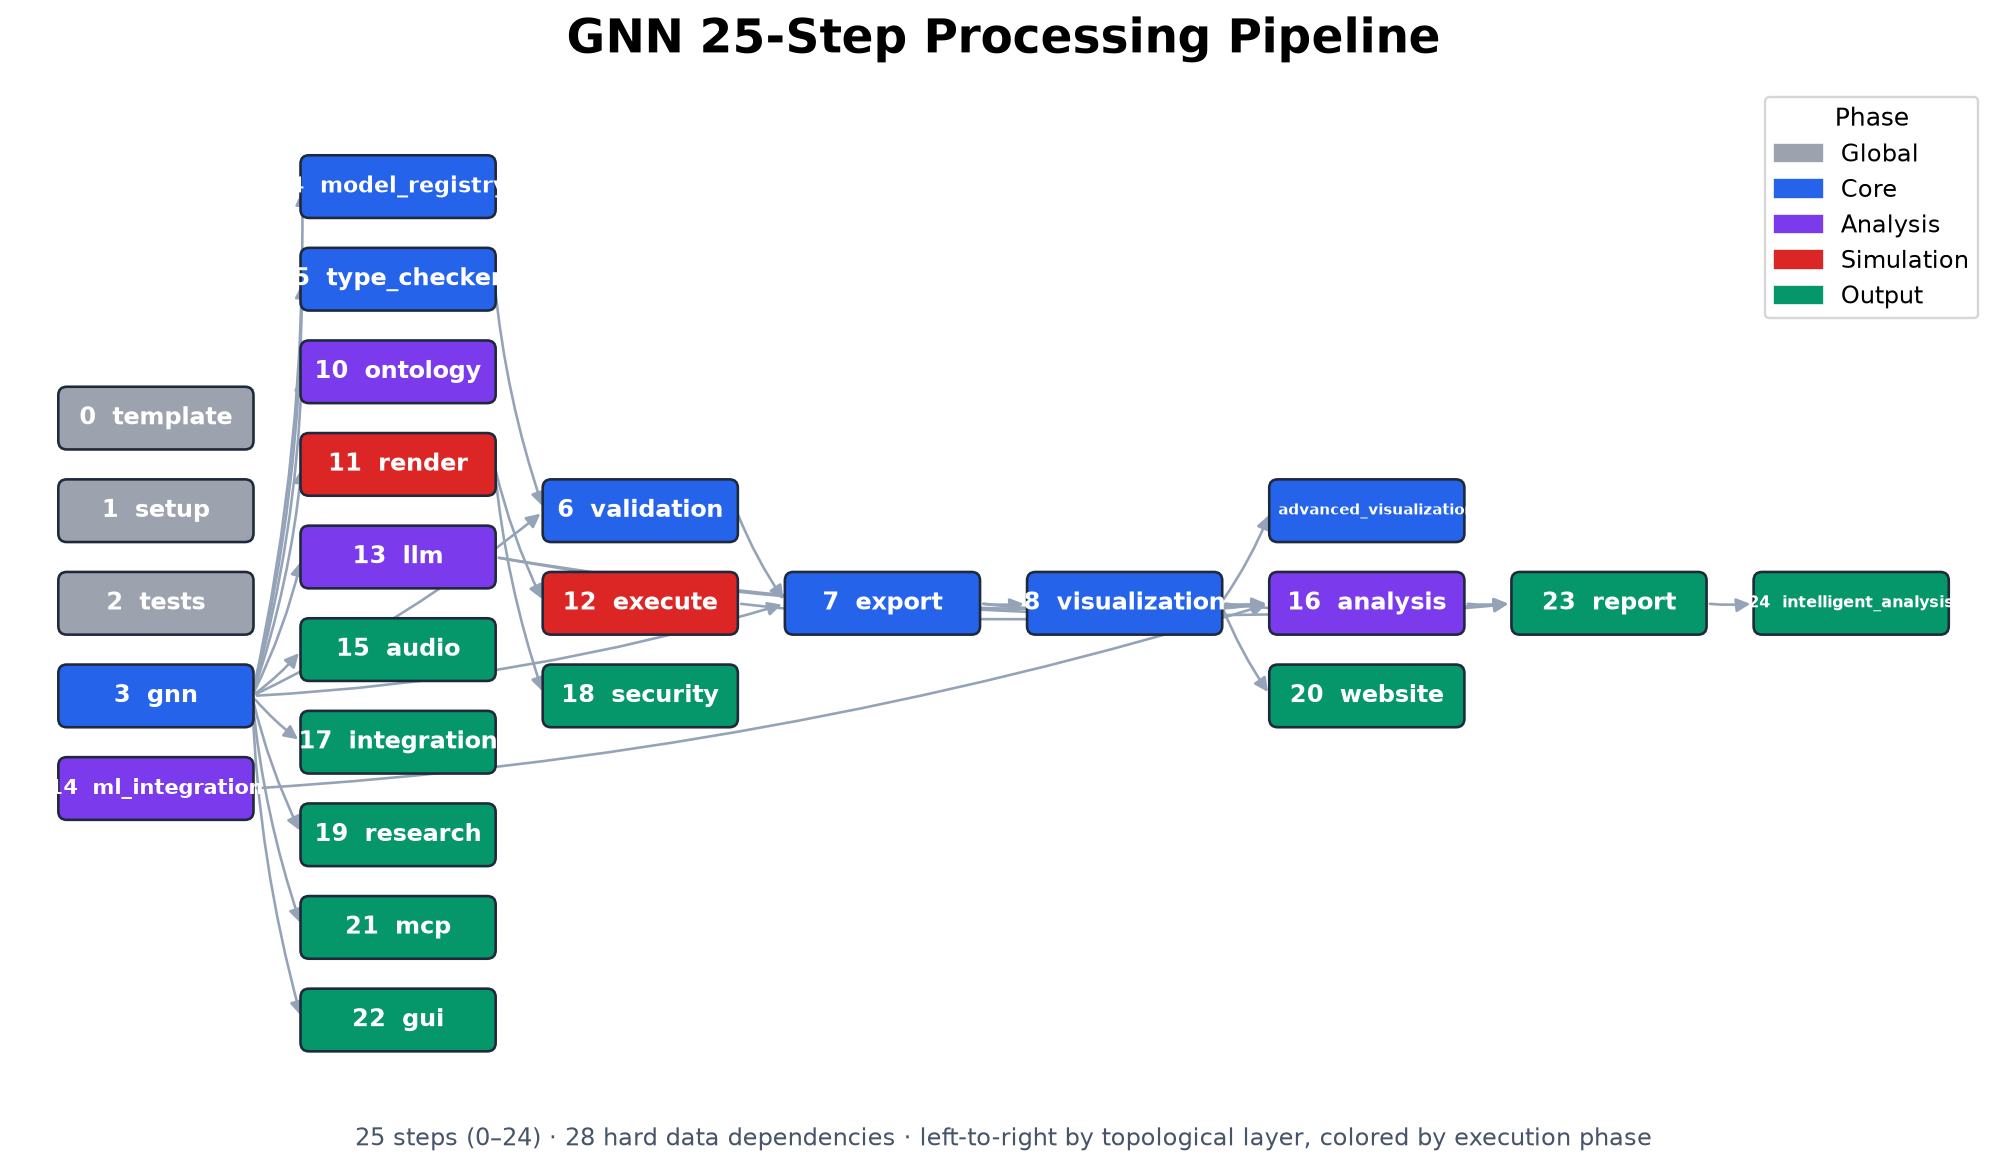
\includegraphics[width=0.9\linewidth,height=0.40\textheight,keepaspectratio,alt={The 25-step GNN processing pipeline as a directed acyclic graph, laid out left to right by topological layer and colored by execution phase (legend, upper right). Each node is the thin step orchestrator under src/gnn/ named in tbl.~; each arrow is a hard data dependency parsed from the Data Dependency Graph block of src/gnn/STEP\_INDEX.md, so any artifact can be traced back to the step that produced it. Parsing (Step 3) fans out to nearly every later step, and analysis (Step 16) collects enrichment from execution, visualization, and the LLM step. The figure is generated from src/gnn/STEP\_INDEX.md at commit ba73789bf; its footer restates the step count, the number of hard dependencies, and the layout rule.}]{../figures/gnn_pipeline_dag.png}
\caption{The 25-step GNN processing pipeline as a directed acyclic
graph, laid out left to right by topological layer and colored by
execution phase (legend, upper right). Each node is the thin step
orchestrator under \protect\texttt{src/gnn/} named in
tbl.~\ref{tbl:pipeline_steps}; each arrow is a hard data dependency
parsed from the Data Dependency Graph block of
\protect\breaktt{src/gnn/STEP\_INDEX.md}, so any artifact can be traced
back to the step that produced it. Parsing (Step 3) fans out to nearly
every later step, and analysis (Step 16) collects enrichment from
execution, visualization, and the LLM step. The figure is generated from
\protect\breaktt{src/gnn/STEP\_INDEX.md} at commit ba73789bf; its footer
restates the step count, the number of hard dependencies, and the layout
rule.}\label{fig:pipeline}
\end{figure}

\end{frame}

\begin{frame}[fragile,allowframebreaks]{The Processing Pipeline}
The per-step responsibilities are enumerated in
tbl.~\ref{tbl:pipeline_steps}; each row names a step and the
transformation it owns within the 0--24 range.

\end{frame}

\begin{frame}[fragile,allowframebreaks]{The Processing Pipeline}
\begin{longtable}[]{@{}
  >{\raggedleft\arraybackslash}p{(\linewidth - 4\tabcolsep) * \real{0.4000}}
  >{\raggedright\arraybackslash}p{(\linewidth - 4\tabcolsep) * \real{0.3000}}
  >{\raggedright\arraybackslash}p{(\linewidth - 4\tabcolsep) * \real{0.3000}}@{}}
\caption{The pipeline steps with the thin orchestrator module that owns
each and the one-line purpose parsed from the master table in
\protect\breaktt{src/gnn/STEP\_INDEX.md}. Read the Step column against
the arrows of fig.~\ref{fig:pipeline}: each row's purpose is the
transformation that module owns, and the table is regenerated from the
index at every build, so it cannot drift from the code it
describes.}\label{tbl:pipeline_steps}\tabularnewline
\toprule\noalign{}
\begin{minipage}[b]{\linewidth}\raggedleft
Step
\end{minipage} & \begin{minipage}[b]{\linewidth}\raggedright
Module
\end{minipage} & \begin{minipage}[b]{\linewidth}\raggedright
Purpose
\end{minipage} \\
\midrule\noalign{}
\endfirsthead
\toprule\noalign{}
\begin{minipage}[b]{\linewidth}\raggedleft
Step
\end{minipage} & \begin{minipage}[b]{\linewidth}\raggedright
Module
\end{minipage} & \begin{minipage}[b]{\linewidth}\raggedright
Purpose
\end{minipage} \\
\midrule\noalign{}
\endhead
0 & \texttt{0\_template.py} & Pipeline template \& initialization \\
1 & \texttt{1\_setup.py} & Environment setup \& UV dependency install \\
2 & \texttt{2\_tests.py} & Test suite execution (pytest) \\
3 & \texttt{3\_gnn.py} & GNN file discovery \& multi-format parsing \\
4 & \breaktt{4\_model\_registry.py} & Model versioning \& registry
management \\
5 & \breaktt{5\_type\_checker.py} & GNN type validation \& resource
estimation \\
6 & \texttt{6\_validation.py} & Consistency \& semantic quality
checking \\
7 & \texttt{7\_export.py} & Multi-format export (JSON, XML, GraphML,
GEXF, Pickle) \\
8 & \breaktt{8\_visualization.py} & Graph \& matrix visualization
generation \\
9 & \breaktt{9\_advanced\_viz.py} & Interactive / advanced visualization
(Plotly, D3) \\
10 & \texttt{10\_ontology.py} & Active Inference ontology processing \&
validation \\
11 & \texttt{11\_render.py} & Code generation for simulation
frameworks \\
12 & \texttt{12\_execute.py} & Execute rendered simulation scripts \\
13 & \texttt{13\_llm.py} & LLM-enhanced analysis \& model
interpretation \\
14 & \breaktt{14\_ml\_integration.py} & Machine learning integration \&
model training \\
15 & \texttt{15\_audio.py} & Audio sonification generation (SAPF) \\
16 & \texttt{16\_analysis.py} & Statistical analysis \& cross-simulation
aggregation \\
17 & \breaktt{17\_integration.py} & System integration \& cross-module
coordination \\
18 & \texttt{18\_security.py} & Security validation \& generated code
scanning \\
19 & \texttt{19\_research.py} & Research tools \& literature
references \\
20 & \texttt{20\_website.py} & Static HTML website generation \\
21 & \texttt{21\_mcp.py} & Model Context Protocol processing \& tool
registration \\
22 & \texttt{22\_gui.py} & Interactive GNN constructor GUI \\
23 & \texttt{23\_report.py} & Comprehensive analysis report
generation \\
24 & \breaktt{24\_intelligent\_analysis.py} & AI-powered pipeline
analysis \& executive reports \\
\bottomrule\noalign{}
\end{longtable}

\end{frame}

\begin{frame}[fragile,allowframebreaks]{The Processing Pipeline}
This staged design keeps the architecture modular. The implementation is
organized into 44 source packages, one cluster of responsibilities per
concern, and is documented across 624 documentation files so that each
step's contract, inputs, and outputs are specified independently of the
others. New backends or analyses attach to the graph by declaring their
dependencies rather than by editing a monolith, and the deterministic
step ordering means a model processed today yields the same artifacts
when reprocessed tomorrow. The pipeline is kind-agnostic in its plumbing
and kind-aware at its edges: parsing, validation, and export operate on
whatever the file declares, while the rendering and execution steps
consult the classification of sec.~\texttt{sec:model\_kinds} to decide which
backends a given model can reach and record, explicitly, the ones it
cannot.
\end{frame}

\subsection{The Triple Play}\label{the-triple-play}

\begin{frame}[fragile,allowframebreaks]{The Triple Play}
The reason for separating a single written language from a multi-stage
pipeline is the design goal GNN calls the Triple Play: one model
specification, three coordinated modes of existence. The same GNN text
is simultaneously a human-readable model description, a set of graphical
visualizations of its state space and factor structure, and an
executable cognitive model that can be run as a simulation.
fig.~\ref{fig:triple_play} depicts these three faces and the shared
specification at their center.

\end{frame}

\begin{frame}[fragile,allowframebreaks]{The Triple Play}
\begin{figure}
\centering
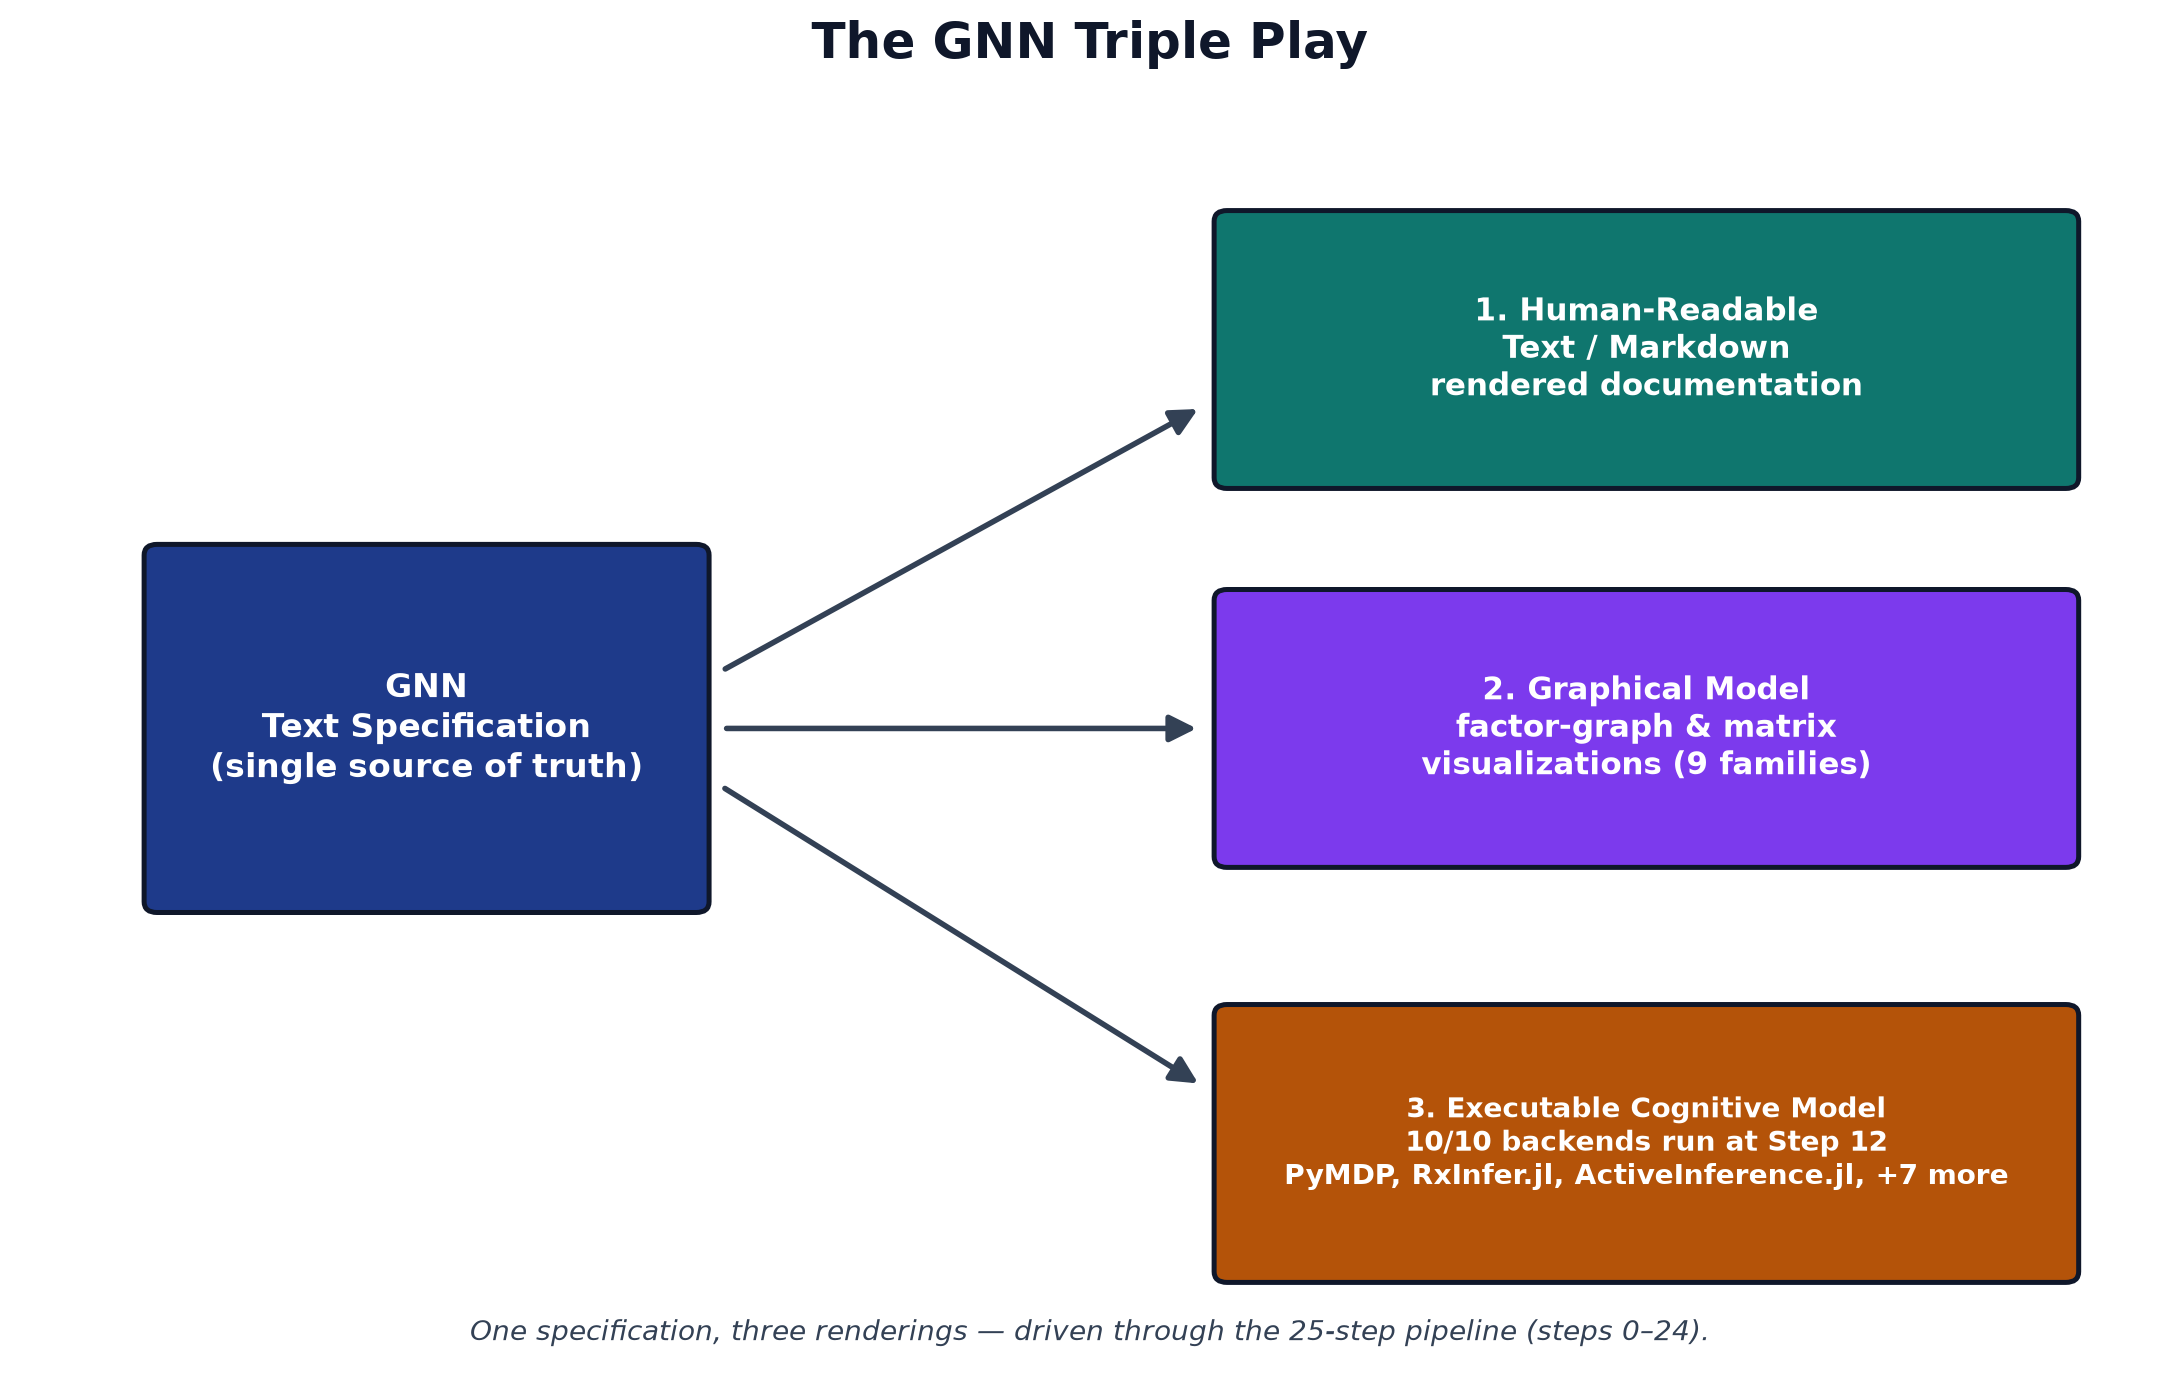
\includegraphics[width=0.7\linewidth,height=0.40\textheight,keepaspectratio,alt={The Triple Play: one GNN text specification (left) and its three coordinated projections (right) --- the human-readable text form, graphical model visualizations, and executable simulation code. All three arrows originate at the same source box because all three projections are generated from one parsed document, which is why they cannot drift apart; the executable node states that 9 of 9 registered backends run at Step 12 and previews three of them by name. Counts are producer tokens at commit ba73789bf, and the panel is generated by scripts/manuscript\_fig\_triple\_play.py. Take-away: a model is authored once and then read, seen, and run from that single source.}]{../figures/gnn_triple_play.png}
\caption{The Triple Play: one GNN text specification (left) and its
three coordinated projections (right) --- the human-readable text form,
graphical model visualizations, and executable simulation code. All
three arrows originate at the same source box because all three
projections are generated from one parsed document, which is why they
cannot drift apart; the executable node states that 9 of 9 registered
backends run at Step 12 and previews three of them by name. Counts are
producer tokens at commit ba73789bf, and the panel is generated by
\protect\breaktt{scripts/manuscript\_fig\_triple\_play.py}. Take-away: a
model is authored once and then read, seen, and run from that single
source.}\label{fig:triple_play}
\end{figure}

\end{frame}

\begin{frame}[fragile,allowframebreaks]{The Triple Play}
Each face is generated from the same source, so they cannot drift apart.
The text is the contract a researcher reads and reviews; the
visualizations expose the factor-graph structure for inspection and
communication; and the executable rendering lets the identical model be
simulated across inference frameworks, connecting the written
specification to the discrete message-passing libraries for categorical
Active Inference (Heins et al. 2022), to the reactive message-passing
and probabilistic-programming engines that carry the linear-Gaussian
kind, and to the broader tooling ecosystem for compositional model
representation (Felice et al. 2021). Because all three derive from one
parsed document, GNN turns a model from a static artifact into a live
object that can be read, seen, and run without re-encoding it for each
purpose (Smith et al. 2022). The Triple Play holds per kind: each of the
three faces is generated from the same classification the pipeline
\end{frame}

\begin{frame}[fragile,allowframebreaks]{The Triple Play}
computed at parse time, so the diagram a reader sees, the notation a
reviewer diffs, and the program a backend executes are all projections
of one declared model kind rather than three loosely coupled guesses
about what the file meant.
\end{frame}

\end{document}
